\documentclass[titlepage=true]{scrartcl}

\input{header/zusammenfassung}
\input{header/hyperref}
\usepackage{multicol}
\usepackage{caption}
\usepackage{subcaption}
\usepackage{tikz}
\usepackage{rotating}
\usepackage{circuitikz}

\setDefaultArrayStretch{1.8}

\title{MikroelSys1}
\author{Jürg Rast}

\begin{document}
% \begin{titlepage}
% 	\thispagestyle{empty}
% 	\maketitle
% \end{titlepage}

\tableofcontents
\newpage

\section{CMOS Technologie\skript{Kap. 3}}

\section{Schaltungselemente in CMOS\skript{Kap. 4}}
Absolutwerte von Widerständen und Kapazitäten können um mehr als $\pm 20\%$ Abweichen! Viel genauer lassen sich Verhältnisse herstellen, dort sind Toleranzen von
unter $1\%$ üblich.

\subsection{Kapazitäten}
Es gibt im wesentlichen drei unterschiedliche Arten von Kapazitäten, welche in einem CMOS-Chip realisiert werden können: 
Poly-Poly-Kapazität ($C'' \approx 1fF/\mu m^2$),
MOS-Kapazität ($C'' \approx 10fF/\mu m^2$),
MIM-Kapazität (Metall-Isolator-Metall, $C'' \approx 1fF/\mu m^2$). $C''$ bezeichnet dabei die spezifische Kapazität pro Flächeneinheit.
Der Plattenabstand $d$ ist meist durch die Herstellung gegeben.

\begin{tabularx}{\linewidth}{|l|X|}
	\hline
	Elektrische Feldkonstante	& $\epsilon_0 = 8.85 \cdot 10^{-12} F/m$
	\\ \hline
	Kapazität/Fläche	& $C'' = \cfrac{\epsilon}{d} = \cfrac{\epsilon_0 \epsilon_r}{d}$
	\\ \hline
	Kapazität & $C = C'' \cdot A$
	\\ \hline
\end{tabularx}

\subsection{Widerstände}
Widerstände in CMOS sind meist unerwünscht da sie viel Platz brauchen und viel Wärme entsteht. Sollte trotzdem ein
Widerstand erforderlich sein, so lässt so ist er über seine Breite und Länge zu definieren:
\[
	R = R_\diamond \frac{L}{W}
\]

\begin{tabularx}{0.8\linewidth}{|l|l|X|l|l|}
	\hline
	\multicolumn{5}{|c|}{\textbf{Typische Werte für Widerstände}}
	\\ \hline
	Poly-Widerstand & $R \approx 10 \Omega/\diamond$ & & HR-Poly-Widerstand & $R \approx 1k\Omega/\diamond$
	\\ \hline
	P-Diffusions-Widerstand & $R \approx 100\Omega/\diamond$ & & N-Diffusions-Widerstand & $R \approx 100\Omega/\diamond$
	\\ \hline
	N-Well-Widerstand & $R \approx 1k\Omega/\diamond$ & & &
	\\ \hline
\end{tabularx}

\section{MOS-Transistoren\skript{Kap. 5}}

% \subsection{Allgemeine Begriffe und Formeln}
%TODO: was ist hier noch nötig?

\subsection{Bestimmung des Arbeitsbereichs}

\begin{enumerate}
	\item Bestimmung ob weak, moderate oder strong inversion.
	\item Berechnen der Sättigungsspannung.
	\item Wenn $V_{DS} > V_{DS,sat}$, $\Rightarrow$ gesättigt.
\end{enumerate}

\begin{tabular}{|l|l|l|}
	\hline
	\textbf{Arbeitsbereich}	& \textbf{Bedingung}					& \textbf{Sättigungspannung}
	\\ \hline
	weak inversion			& $0 < V_{GS} < V_T - 60mV$				& $V_{DS,sat} \approx 5\Phi_t \approx 130mV \quad \text{(bei } T = 300K \text{)}$ \\
	$I_D' < I_M'$			&										& $V_{GS} = V_{M} + h_{M} \cdot \Phi_t \cdot 																\ln{\frac{I_{D}}{\frac{W}{L} \cdot I_{M}}}$ 
	\\ \hline
	moderate inversion		& $V_T - 60mV < V_{GS} < V_T + 160mV$	& \\
	$I_M' < I_D' < I_H'$ 	& 										&
	\\ \hline
	strong inversion		& $V_T + 160mV < V_{GS} $				& $V_{DS,sat} = V_{GS} - V_T = \sqrt{\frac{{2 I_{D}}}{\beta}} = \sqrt{\frac{2 I_{D}}{\frac{W}{L} \cdot \beta_{0}}}$
	\\ 
	$I_H' < I_D'$ & & \\ \hline
\end{tabular} \\

mit $I_D = \frac{W}{L} I_D'$ \hspace{5mm} und \hspace{5mm} $\Phi_t = \frac{kT}{e}$, wobei $k = 1.38 \cdot 10^{-23} \frac{J}{K}$, und $e = 1.6 \cdot 10^{-19}C$ \\

\subsection{Kennlinien}
\subsubsection{Ausgangskennlinie}
\begin{minipage}{8cm}
	\centering
	\includegraphics[width=7cm]{images/Ausgangskennlinie.png}
\end{minipage}
\begin{minipage}{10cm}
	\textbf{Gesättigt}, Stromquellen-Betrieb:\\
	Geraden horizontal, dann ist $r_{DS}=\infty$ (idealer Transistor). \\
	Anstieg der Geraden entspricht Ausgangsleitwert $g_0$ bzw. Ausgangswiderstand $r_{DS}$. \\
	
	\textbf{Ungesättigt}, Widerstandsbetrieb: \\
	Je steiler die Gerade, desto kleiner $r_{DS}$. \\
\end{minipage}

\subsubsection{Transferkennlinie}
{	\centering
		\adjustbox{scale=0.7}{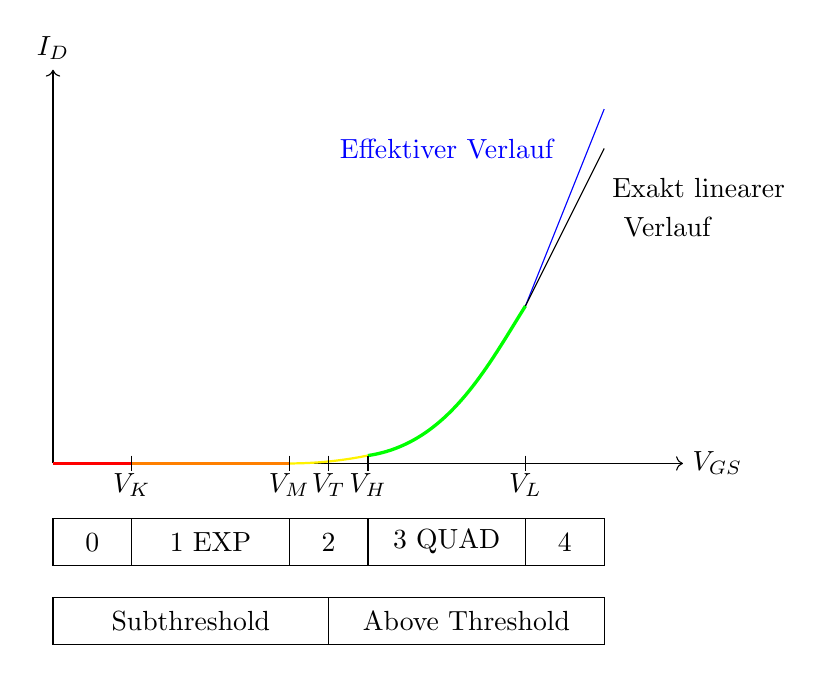
\begin{tikzpicture}

\draw [->] (0,0) -- (0,5) node [anchor=south] {$I_D$};
\draw [->] (0,0) -- (8,0) node [anchor=west] {$V_{GS}$};

\draw [color=red, thick] (0,0) -- (1,0);
\draw [color=orange, very thick] (1,0) -- (3,0);
\draw [color=yellow, thick] (3,0) arc (-90:-78:5);
\draw [color=green, very thick] (4.0,0.1) .. controls (5,0.25) and (5.5,1.2) .. (6,2);
\draw [color=blue] (6,2) -- (7,4.5);
\draw (6,2) -- (7,4);

\node [color=blue] at (5,4) {Effektiver Verlauf}; 
\node at (8.2,3.5) {Exakt linearer};
\node at (7.8,3) {Verlauf};


\foreach \x in {1,3,4,6} {
	\draw (\x,0.1) -- (\x,-0.1);
	\draw (\x,-0.7) -- (\x,-1.3);
}

\draw (3.5,0.1) -- (3.5,-0.1);

\draw (0,-0.7) rectangle (7,-1.3);

\node at (1,0) [anchor=north] {$V_K$};
\node at (3,0) [anchor=north] {$V_M$};
\node at (3.5,0) [anchor=north] {$V_T$};
\node at (4,0) [anchor=north] {$V_H$};
\node at (6,0) [anchor=north] {$V_L$};

\node at (0.5,-1) {0};
\node at (2,-1) {1 EXP};
\node at (3.5,-1) {2};
\node at (5,-1) {3 QUAD};
\node at (6.5,-1) {4};

\draw (0,-1.7) rectangle (7,-2.3);
\draw (3.5,-1.7) -- (3.5,-2.3);
\node at (1.75,-2) {Subthreshold};
\node at (3.5+1.75,-2) {Above Threshold};
\end{tikzpicture}}
	\qquad\qquad
		\includegraphics[width=7cm]{images/Transferkennlinie.png}
} \\

\setArrayStretch{1.1}
\begin{tabular}{|lp{3cm}|p{6cm}|p{8cm}|}
	\hline
	& \textbf{Ausgangs\-strom\-bereich} & \textbf{Mathematische Charakterisierung} & \textbf{Zugrundeliegender physikalischer Effekt}
	\\ \hline
	\cellcolor{red!70}
	0 
	& Leckstrombereich (LECK) 
	& $I_D$ erreicht Minimalwert, der nicht weiter unterschritten werden kann
	& Drain-Substratdiode und Source-Substratdiode haben Leckströme im Substrat
	\\ \hline
	\cellcolor{orange!70}
	1
	& Exponentieller Bereich (EXP)
	& $I_D$ steigt exponentiell mit $V_{GS}$
	& Kanal zeigt schwache Inversion (Beim n-Kanal-Transistor: Ursprünglich p-leitender Kanal ist schwach n-leitend)
	\\ \hline
	\cellcolor{yellow!70}
	2
	& Schwellen Bereich (MOD)
	& Keine "`handlichen"' Formel für $I_D$ vorhanden
	& Kanal zeigt moderate Inversion (Kanalzustand liegt zwischen schwacher und starker Inversion)
	\\ \hline
	\cellcolor{green!70}
	3
	& Quadratischer Bereich (QUAD)
	& $I_D$ steigt quadratisch mit $V_{GS}$
	& Kanal zeigt starke Inversion (Beim n-Kanal-Transistor: Ursprünglich p-leitender Kanal wirk stark n-leitend)
	\\ \hline
	\cellcolor{blue!70}
	4
	& Linearer Bereich (LIN)
	& $I_D$ steigt annähernd linear mit $V_{GS}$ (halb QUAD, halb LIN)
	& Geschwindigkeitsänderung der Ladungsträger im Kanal (die Ladungsträger können nicht weiter beschleunigt werden)
	\\ \hline
\end{tabular}
\resetArrayStretch


\subsection{Drainstromgleichungen}
\setArrayStretch{1.4}
\begin{tabular}{|p{3.8cm}|l|l|}
	\hline
		\textbf{Ausgangsstrom} 
		& \multicolumn{2}{c|}{\textbf{Ausgangsspannungsbereich} ($V_{DS}$-Bereich)}
	\\
		($I_D-, V_{GS}$-Bereich)
		& Transistor ungesättigt ($|V_{DS}| < |V_{DS,sat}|$)
		& Transistor gesättigt ($|V_{DS}| > |V_{DS,sat}|$)
	\\ \hline
		\multicolumn{3}{|c|}{\textbf{n-Kanal Transistor}}
	\\ \hline
		EXP-Bereich \newline (weak inversion)
		& $I_D = I_M e^{\frac{V_{GS}-V_M}{n_M \Phi_t}} (1-e^{\frac{-V_{DS}}{\Phi_t}}) (1 + \lambda V_{DS})$
		& $I_D = I_M e^{\frac{V_{GS}-V_M}{n_M \Phi_t}} (1 + \lambda V_{DS})$
	\\ \hline
		QUAD-Bereich \newline (strong inversion)
		& $I_D = B [(V_{GS} - V_T) V_{DS} - \frac{V_{DS}^2}{2}] (1 + \lambda V_{DS})$
		& $I_D = \frac{\beta}{2}(V_{GS} - V_T)^2 (1 + \lambda V_{DS})$
	\\ \hline
		\multicolumn{3}{|c|}{\textbf{p-Kanal Transistor}}
	\\ \hline
		EXP-Bereich \newline (weak inversion)
		& $I_D = I_M e^{-\frac{V_{GS}-V_M}{n_M \Phi_t}} (1-e^{\frac{-V_{DS}}{\Phi_t}}) (1 - \lambda V_{DS})$
		& $I_D = I_M e^{-\frac{V_{GS}-V_M}{n_M \Phi_t}} (1 - \lambda V_{DS})$
	\\ \hline
		QUAD-Bereich \newline (strong inversion)
		& $I_D = -B [(V_{GS} - V_T) V_{DS} - \frac{V_{DS}^2}{2}] (1 - \lambda V_{DS})$
		& $I_D = -\frac{\beta}{2}(V_{GS} - V_T)^2 (1 - \lambda V_{DS})$
	\\ \hline
\end{tabular} \\

Wird die Kanallängenmodulation vernachlässigt, kann einfach der $(1 - \lambda V_{DS})$ Term weggelassen werden. \\

\subsection{Kleinsignal-Ersatzschaltbild}
\begin{figure}[htbp]
        \centering
        \begin{subfigure}[b]{5cm}
                \centering
                \adjustbox{scale=0.7}{\begin{circuitikz}[american, european resistors]
	\draw (1.5,0) node[circ, name=G] {} node[right] {G};
	\draw (4,0) node[circ, name=D] {} node[right] {D};
	\draw (4,-2) node[circ, name=S] {} node[right] {S};
	\draw (0,-2) -- (S);
	\draw (G) -- +(-1.5,0);
	\draw (3,0) to[R=$r_{DS0}$] +(0,-2);
	\draw (0,-2) to[V] ++(0,2) ;
	\draw (0,-2) -- + (0,-0.2) node[ground] {};
	\draw (D) -- +(-1,0);
	\draw[->, thick] (-0.9, -0.2) -- +(0,-1.4) node[midway, left] {$V_{GS}$};
\end{circuitikz}}
                \caption{Widerstandsbetrieb}
        \end{subfigure} \qquad \qquad
        \begin{subfigure}[b]{5cm}
                \centering
                \adjustbox{scale=0.7}{\begin{circuitikz}[american, european resistors]
	\draw (1.5,0) node[circ, name=G] {} node[right] {G};
	\draw (5,0) node[circ, name=D] {} node[right] {D};
	\draw (5,-2) node[circ, name=S] {} node[right] {S};
	\draw (0,-2) -- (S);
	\draw (G) -- +(-1.5,0);
	\draw (4,0) to[R=$r_{DS}$] +(0,-2);
	\draw (3,0) to[I,mirror,l=$g_mV_{GS}$] +(0,-2);
	\draw (0,-2) to[V] ++(0,2) ;
	\draw (0,-2) -- + (0,-0.2) node[ground] {};
	\draw (D) -- ++(-1,0) to[short, i_=$I_D$] +(-1,0);
	\draw[->, thick] (-0.9, -0.2) -- +(0,-1.4) node[midway, left] {$V_{GS}$};
\end{circuitikz}}
                \caption{Stromquellenbetrieb, PI-ESB}
        \end{subfigure} \qquad \qquad
        \begin{subfigure}[b]{5cm}
                \centering
                \adjustbox{scale=0.7}{\begin{circuitikz}[american, european resistors]
	\draw (1.5,0) node[circ, name=G] {} node[above] {G};
	\draw (5,2) node[circ, name=D] {} node[right] {D};
	\draw (5,-2) node[circ, name=S] {} node[right] {S};

	\draw (G) -- +(-1.5,0);
	
	\draw (G)  -- (3,0);
	\draw (3,2) to[I,mirror,l=$g_mV_{GS}$] (3,0);
	\draw (3,2) -- (D);
	
	\draw (3,0) to[R={$R_s$},mirror] +(0,-2);
	\draw (0,-2) to[V] ++(0,2) ;
	\draw (0,-2) -- + (0,-0.2) node[ground] {};
	\draw (S) -- (0,-2);
	\draw[->, thick] (-0.9, -0.2) -- +(0,-1.4) node[midway, left] {$V_{GS}$};
	
	\draw (4.2,2) to[R=$r_{DS}$,mirror] (4.2,-2);
	
\end{circuitikz}}
                \caption{Stromquellenbetrieb, T-ESB}
        \end{subfigure}        
\end{figure}
\subsection{Kleinsignalparameter}
\begin{tabularx}{\linewidth}{|X|l|l|}
	\hline
		& \textbf{Transistor ungesättigt} & \textbf{Transistor gesättigt} 
	\\ \hline
		& Kanalwiderstand bei $V_{DS}=0$:
		& Kanalwiderstand:
	\\
		& $r_{DS0} = \frac{dV_{DS}}{dI_D}|_{V_{DS}=0} = \frac{\Phi_t}{I_{D0}}$
		& $r_{DS} = \frac{dV_{DS}}{dI_D} = \frac{V_A + V_{DS}}{I_D} \approx \frac{V_A}{I_D}$
	\\ weak
		& Kanalwiderstand bei $V_{DS} = 0V \dots V_{DS,sat}$:
		& 
	\\ inversion
		& $r_{DS} = \frac{dV_{DS}}{dI_D} \approx \frac{\Phi_t}{I_D} e^{\frac{V_{DS}}{\Phi_t}}$ (ungenau, kaum benötigt)
		&
	\\ \cline{2-3}
		& $g_m$ nicht benötigt
		& Steilheit
	\\
		& 
		& $g_m =  \frac{dI_D}{V_{GS}} = \frac{I_D}{n_m \Phi_t}$	
	\\ \hline
		& Kanalwiderstand bei $V_{DS}=0$:
		& Kanalwiderstand:
	\\
		& $r_{DS0} = \frac{dV_{DS}}{dI_D}|_{V_{DS}=0} = \frac{1}{\beta (V_{GS} - V_T) (1 + \lambda V_{DS})}$
		& $r_{DS} = \frac{dV_{DS}}{dI_D} = \frac{V_A + V_{DS}}{I_D} \approx \frac{V_A}{I_D}$
	\\ strong
		& Kanalwiderstand bei $V_{DS} = 0V \dots V_{DS,sat}$:
		& $r_{DS} = \frac{dV_{DS}}{dI_D}|_{V_{DS}=0} = \frac{1}{\beta [(V_{GS} - V_T)-V_{DS}] (1 + \lambda V_{DS})}$
	\\ \cline{2-3} inversion
		& $g_m$ nicht benötigt
		& Steilheit (zwei Formeln)
	\\
		&
		& $g_m = \frac{dI_D}{V_{GS}} = \beta (V_{GS} - V_T) (1 + \lambda V_{DS})$
	\\
		&
		& $g_m = \frac{dI_D}{V_{GS}} = \sqrt{2 I_D \beta (1 + \lambda V_{DS})} $
	\\ \hline
\end{tabularx}

\subsection{Parameter}

\begin{longtable}{|l|l|p{11cm}|}
	\hline
		$V_{DS,sat}$	& Sättigungsspannung	&
	\\ \hline
		$a_A$			& Early-Faktor			&
	\\ \hline
		$V_T$ & Schwellenspannung &
		Typisch $0.6V$ beim n-Kanal, resp. $-0.6V$ beim p-Kanal. $V_T$ ist stark von der Source-Bulk-Spannung abhängig (Body-Effekt):
		\[ 
			V_T = V_{T0} \pm \Delta V_T \quad \text{mit} \quad \Delta V_T = \gamma(\sqrt{V_{SB} \pm \Phi_0} -\sqrt{\Phi_0})
		\]
		positives Vorzeichen für n-Kanal, negatives für p-Kanal, $\gamma_N \approx 0.6\sqrt{V}$, $\gamma_P \approx 0.5\sqrt{V}$, $\Phi_{0} = 0.6V$ 
	\\ \hline
		$\Phi_t$ & Temperaturspannung &
		\[
			\Phi_t = V_{Temp} = \frac{kT}{e} = 86.2 \frac{\mu V}{K}T
		\]
		somit ist $\Phi_t = 25.9mV$ bei $T=300^\circ K$ bzw. $27^\circ C$
	\\ \hline
		$I_M$ & Drainstrom &
		Drainstrom an der Grenze zwischen schwacher und moderater Inversion.
		\[
			I_M = \frac{W}{L} \cdot I_M'
		\]
		$I_M'$ ist der spezifische Drainstrom an der Grenze
	\\ \hline
		$n_M$ & Unterschwellen-Neigungsfaktor &
		Der Faktor $n_m$ ist von der Source-Bulk-Spannung $V_{SB}$ abhängig:
		\[
			n_M = 1 + \frac{\gamma}{2 \sqrt{V_{SB} + \Phi_0}}
		\]
		mit $\Phi_0 = 2 \Phi_F \approx 0.6V$. 
		Für $V_{SB} = 0$ erhalten wir $n_M=1.39$. Häufig wird ein Wert von $n_M \approx 1.5$ angegeben.
	\\ \hline
		$V_A$			& Early-Spannung		& $V_A \approx a_A \cdot L$ \quad $V_{A}$ ist immer positiv
	\\ \hline
		$\lambda$ & Kanallängen-Modulationsfaktor &
		inverser Wert der Early-Spannung
		\[
			\lambda = \frac{1}{V_A} \approx \frac{1}{a_A L}
		\]
		Der MOS-Transistor wird vielfach mit $\lambda = 0$ idealisiert, was die Handrechnung vereinfacht.
	\\ \hline
		$B, \beta$ & Transkondukdanz &
		Steilheit, Verstärkungsfaktor. Dieser Faktor ist im gesättigten und ungesättigten Betrieb \textbf{grundsätzlich verschieden}. Es gilt: $\beta = \frac{W}{L} \beta_0 = \frac{W}{L} \mu C_{ox}''$. 
	\\ \hline
		$g_{m}$	& Transkonduktanz & Steilheit oder Gate-Steilheit. Beschreibt Zusammenhang zwischen $I_{DS}$ und $V_{GS}$. Mass für die Verstärkung.
	\\ \hline
		$g_{mb}$ & Body-Transkonduktanz & Beschreibt Wirkung des Body-Effekts. Nur im gesättigtem Stromquellenbetrieb von Bedeutung. Berechnung siehe Zbinden Formeln.
	\\ \hline
		$g_{0}$ & Ausgangsleitwert &
	\\ \hline
		$r_{DS}$ & Ausgangswiderstand & $r_{DS} = \frac{1}{g_0} \approx \frac{\Delta 	V_{DS}}{\Delta I_D} \quad 
													  \text{oder} \quad r_{DS} = \frac{V_A + V_{DS}}{I_{D,real}} \approx \frac{V_A}{I_D} $ 
	\\				&			&$V_{A}, V_{DS}, I_{D,real}$ immer im Betrag  
	\\ \hline
		$r_{s}$	& innerer Source-Widerstand & $r_{s} = \frac{1}{g_{m}}$
	\\ \hline
\end{longtable}


\section{Grundschaltungen mit MOS-Transistoren}

\section{MOS-Diode\skript{Kap. 7}}
Für Kennlinien der MOS-Dioden siehe Abbildung \ref{fig:diodenKennlinien}. Die MOS-Diode funktioniert im Stromquellenbetrieb.
\begin{figure}[h]
	\centering
	\begin{subfigure}[b]{5cm}
		\centering
		\adjustbox{scale=0.7}{\begin{circuitikz}[european voltages]
	\draw (0,0) to[full diode, i=$I_D$] (0,-2);
	\draw[->, thick] (-0.7,-0.2) -- (-0.7,-1.8) node[midway, left] {$V_D$};
\end{circuitikz}}
		\caption{Ideale Diode ($V_F = V_{F0}$)}
	\end{subfigure}
	\begin{subfigure}[b]{4cm}
		\centering
		\adjustbox{scale=0.7}{\begin{circuitikz}[european voltages]
	\draw (0,0) to[full diode, i=$I_D$] (0,-2);
	\draw[->, thick] (-0.7,-0.2) -- (-0.7,-1.8) node[midway, left] {$V_D$};
\end{circuitikz}}
		\caption{Reale Diode}
	\end{subfigure} \quad
	\begin{subfigure}[b]{4cm}
		\centering
		\adjustbox{scale=0.7}{\begin{circuitikz}[european voltages]
	\ctikzset{tripoles/mos style/arrows}
	\draw (0,-1) to[Tnmos, n=n1] (0,0);
	\draw (n1.source) to[short, i=$I_D$] (0,-2);
	\draw (n1.gate) |- (n1.drain) -- +(0,0.5);
	\draw[->, thick] (-1.2,0.5) -- (-1.2,-1.5) node[midway, left] {$V_{GS}$};
\end{circuitikz}}
		\caption{n-Kanal}
	\end{subfigure}
	\begin{subfigure}[b]{4cm}
		\centering
		\adjustbox{scale=0.7}{\begin{circuitikz}[european voltages]
	\ctikzset{tripoles/mos style/arrows}
	\draw (0,-1) to[Tpmos, n=n1] (0,0);
	\draw (n1.source) to[short, i<=$I_D$] +(0,0.4);
	\draw (n1.gate) |- (n1.drain) -- +(0,-0.5);
	\draw[->, thick] (0.5,0) -- +(0,-1.5) node[midway, right] {$V_{GS}$};
\end{circuitikz}}
		\caption{p-Kanal}
	\end{subfigure}
	\hspace{1.5cm}
	
	\begin{subfigure}[b]{4cm}
		\adjustbox{scale=0.7}{\begin{tikzpicture}
	\draw[->] (0,0) -- (0,3.5) node[left] {$I_D$};
	\draw[->] (0,0) -- (3.5,0) node[below] {$V_D$};
	\draw (0, 0.04) -- ++(2,0) -- +(0,3);
\end{tikzpicture}}
	\end{subfigure} \quad
	\begin{subfigure}[b]{4cm}
		\centering
		\adjustbox{scale=0.7}{\begin{tikzpicture}
	\draw[->] (0,0) -- (0,3.5) node[left] {$I_D$};
	\draw[->] (0,0) -- (3.5,0) node[below] {$V_D$};
	\draw (0, 0.04) -- ++(1.2,0);
	\draw (1.2,0.04) .. controls (1.5,0.04) and (1.7,2.8) .. (1.7,2.8);
	\draw (2,3.3) node {$I_D = I_S (e^{\frac{V_D}{\Phi_t}}  -1)$};
\end{tikzpicture}}
	\end{subfigure} \qquad
	\begin{subfigure}[b]{8cm}
		\centering
		\adjustbox{scale=0.7}{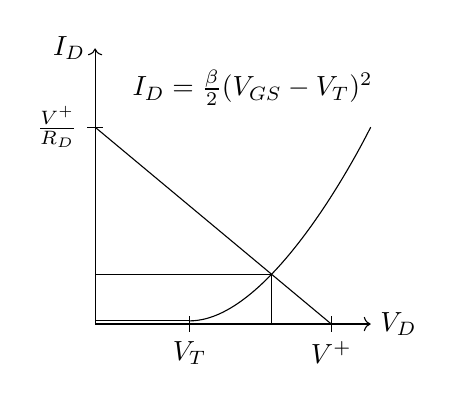
\begin{tikzpicture}
	\draw[->] (0,0) -- (0,3.5) node[left] {$I_D$};
	\draw[->] (0,0) -- (3.5,0) node[right] {$V_D$};
	\draw (0, 0.04) -- ++(1.2,0);
	\draw (1.2,0.04) .. controls (2.3,0.04) and (3.5,2.5) .. (3.5,2.5);
	\draw (2,3) node {$I_D = \frac{\beta}{2}(V_{GS} -V_T)^2$};
	\draw (1.2,0.1) -- +(0,-0.2) node[below] {$V_T$};
	\draw (0,0.63) -- ++(2.242,0) --  +(0,-0.63);
	\draw (0,2.5) -- (3,0);
	\draw (-0.1, 2.5) -- +(0.2,0);
	\draw (-0.1, 2.5) node[left] {$\frac{V^+}{R_D}$};
	\draw (3, 0.1) -- +(0, -0.2) node[below] {$V^+$};
\end{tikzpicture}}
	\end{subfigure}			
	\caption{Gegenüberstellung Dioden-Kennlinien}
	\label{fig:diodenKennlinien}
\end{figure}

\begin{figure}[h]
	\centering
	\begin{subfigure}[b]{5cm}
		\centering
		\adjustbox{scale=0.8}{\begin{circuitikz}[american, european resistors]
	\draw (0,0) node[circ, name=G] {} node[left] {G};
	\draw (4,0) node[circ, name=D] {} node[right] {D};
	\draw (4,-2) node[circ, name=S] {} node[right] {S};
	\draw (0,-2) -- (S);
	\draw (G) -- +(3,0);
	\draw (3,0) to[R=$\frac{1}{g_0}$] +(0,-2);
	\draw (2,0) to[I_=$g_m v_{GS}$] +(0,-2);
	\draw (D) to[short, i_=$i_D$] +(-1,0);
	\draw[->, thick] (0, -0.2) -- +(0,-1.6) node[midway, left] {$v_{GS}$};
\end{circuitikz}}
	\end{subfigure} \qquad\qquad
	\begin{subfigure}[b]{3cm}
		\centering
		\adjustbox{scale=0.8}{\input{tikz/mos_diode_ersatzschaltung2}}
	\end{subfigure} \qquad\qquad
	\begin{subfigure}[b]{2cm}
		\centering
		\adjustbox{scale=0.8}{\begin{circuitikz}[american, european resistors]
	\draw (4,0) node[circ, name=D] {} node[right] {D};
	\draw (4,-2) node[circ, name=S] {} node[right] {S};
	\draw (3,-2) -- (S);
	\draw (3,0) to[R=$\frac{1}{g_m}$] +(0,-2);
	\draw (D) to[short, i_=$i_D$] +(-1,0);
\end{circuitikz}}
	\end{subfigure}
	\caption{Ersatzschaltungen der MOS-Diode}
\end{figure}

\begin{tabular}{|l|l|}
	\hline
	Arbeitspunktstrom einer MOS-Diode mit Wiederstandslast $R_D$
	& $I_D = \frac{\beta}{2} (V_{GS} -V_T)^2 = \frac{V^+ - V_{GS}}{R_D} $
	\\ \hline
	$V_{DS}$ einer MOS-Diode bei gegebenem Strom
	& $ V_{DS} = V_T + \sqrt{\frac{2I_D}{\beta(1+\lambda V_{DS})}} \approx V_T + \sqrt{\frac{2I_D}{\beta}} $
	\\ \hline
	Innenwiderstand der MOS-Diode
	& $ r_{MD} = \frac{v_{GS}}{i_D} = \frac{1}{g_m + g_0} \approx \frac{1}{g_m} $
	\\ \hline	
\end{tabular}



\section{MOS-Transistor als Stromquelle\skript{Kap. 8}}

{ \centering
\begin{minipage}{0.49 \linewidth}
	\subsection{Strom einer MOS Stromquelle}
	$I_D=\frac{\beta}{2}\left(V_{GS}-V_T\right)^2 \textcolor{HSRLakeGreen}{(1 + \lambda V_{DS})}
	\approx \frac{\beta}{2}\left(V_{GS}-V_T\right)^2 $
\end{minipage}
\begin{minipage}{0.49 \linewidth}
	\subsection{Sättigungsspannung}
	\textbf{Bei starker Inversion}
	$V_{DS,sat}=V_{GS}-V_t=\sqrt{\frac{2I_d}{\beta}}$\\
	\textbf{Bei schwacher Inversion} $V_{DS,sat}\approx 5 \Phi_t \approx 130mV$
\end{minipage}
}

\begin{tabularx}{\linewidth}{|l|p{3cm}|X|X|}
\hline
Schaltung & Konfiguration & Ausgangswiderstand $r_0$ & Minimale Ausgangsspannung $V_{0,min}$ 
\\ \hline
\adjustbox{valign=t, padding=1ex}{\begin{circuitikz}[scale=0.5, transform shape, european]
\ctikzset{tripoles/mos style/arrows}

\draw (1.5,3) node[nmos] (nmos) {}
	(nmos.G) to (0,3) to [V_=VG] (0,0) node[ground] {}
	(nmos.S) to [R=RS] (1.5,0) node[ground] {}
	(nmos.D) to [R=RL,i<_=ID] (1.5,5.5) node[ocirc] {}
;
\draw [->] (2.5,3.5) -- (2.5,0);
\draw node at (2.5,1.75) [anchor=west] {Vo};
\draw node at (1.5,5.5) [anchor=south] {VDD=V+};
\end{circuitikz}} &
Einfache Quelle mit 1 Transistor &
$r_{out}=r_{iD}=r_{DS}=\frac{1}{g_0}=\frac{V_A+V_{DS}}{I_D}\approx\frac{V_A}{I_D}$ &
$V_0 > V_{0,min} = V_{DS,sat}$ 
\\ \hline
 & Stromquelle mit Source-Widerstand &
$r_{iD}=r_{DS}\left(1+\frac{R_S}{r_S}+\frac{R_S}{r_{DS}}\right)=\frac{1}{g_0}\left(1+g_mR_S\right)+R_S$
& $V_0 > V_{0,min} = R_SI_D+V_{DS,sat}$
\\ \hline
\adjustbox{valign=t, padding=1ex}{\begin{circuitikz}[scale=0.5, transform shape, european]
\ctikzset{tripoles/mos style/arrows}

\draw (3,2) node[nmos] (M1) {}
	(3,4) node [nmos] (M2) {}
	(M1.D) -- (M2.S)
	(M2.D) to [R=RL] (3,6.5) node [ocirc] {}
	(M1.S) to [R=RS] (3,0) node [ground] {}
	(M2.G) to (0,4) to [V=VG2] (0,0) node [ground] {}
	(M1.G) to (1.4,2) to [V=VG1] (1.4,0) node [ground] {}
;
\draw (3.2,4.7) -- (5.5,4.7);
\draw (3.2,2.7) -- (4.5,2.7);
\draw node at (4,5.5) {ro2};
\draw [->] (4,5.3) -- (4,4.7);
\draw node at (4,3.5) {ro2};
\draw [->] (4,3.3) -- (4,2.7);
\draw [->] (5.2,4.5) -- (5.2,0);
\draw node at (5.2,2.25) [anchor=west] {Vo};

\end{circuitikz}} & Stromquelle mit Kaskode &
$r_{out}=r_{o2}\approx\frac{r_{DS}^2}{r_{S2}}=\left(\frac{r_{DS}}{r_S}\right)r_{DS}=\mu\cdot
r_{DS}=\frac{1}{g_{o1}}\cdot\frac{g_{m2}}{g_{o2}}$ & 
$V_{0,min}=V_{G2}-V_{GS2}+V_{DS2,sat}$\newline$V_{0,min}=V_{DS1,sat}+V_{DS2,sat}$\newline$
\left(\text{mit } V_{G2}=V_{DS1,sat}+V_{GS2}\right)$
\\ \hline 
\adjustbox{valign=t, padding=1ex}{\begin{circuitikz}[scale=0.5, transform shape, american]
\ctikzset{tripoles/mos style/arrows}

\draw
	(4,1) node [nmos] (M1) {}
	(2,2) node [nmos, scale=-1] (M3) {}
	(4,3) node [nmos] (M2) {}
	
	(M1.S) to (4,0) node [ground] {}
	(M1.G) to (0.5,1) node [ocirc] {}
	(M1.D) to (M2.S)
	
	(M2.G) to (2,3) node [circ] {}
	(M2.D) to (4,4) node [ocirc] {}
	
	(M3.D) to (2,0) node [ground] {}
	(M3.G) to (4,2) node [circ] {}
	(2,4.5) node [ocirc] {} to [I=IQ] (M3.S)
	(0.5,0) node [ground] {}
;
\draw node at (4,1) [anchor=west] {M1};
\draw node at (2,2) [anchor=east] {M2};
\draw node at (4,3) [anchor=west] {M3};
\draw [->] (0.5,1) -- (0.5,0);
\draw node at (0,0.5) {Vi};
\draw [->] (4,5) -- (4,4);
\draw node at (4,4.5) {ID};
\draw [->] (5,4) -- (5,0) {};
\draw node at (5,2) [anchor=west] {Vo};

\end{circuitikz}} & Stromquelle mit
 geregelter Kaskode &$r_{out} \approx
r_{DS1}\cdot\frac{r_{DS2}}{r_{S2}}\cdot\frac{r_{DS3}}{r_{S3}}=\frac{1}{g_{o1}}\cdot\frac{g_{m2}}{g_{o2}}\cdot\frac{g_{m3}}{g_{o3}}
$ &$V_{O,min}=2V_{DS,sat}$
\\ \hline
\end{tabularx}

\section{MOS Stromspiegel\skript{Kap. 9}}
Ziel: Aus einer einzelnen genauen Strom- oder Spannungsquelle verschiedene genaue Ströme erzeugen.

\begin{tabularx}{\linewidth}{|l|l|X|}
	\hline
	Stromspiegelverhältnis & $n_m$ & $n_m = \frac{I_0}{I_i} = \frac{(\frac{W}{L})_{out}}{(\frac{W}{L})_{in}} \approx \frac{i_0}{i_i}$
	\\ \hline
\end{tabularx}

\subsection{Die wichtigsten Formeln}
\begin{multicols}{2}
	\textbf{Stromspiegelverhältnis}
	\[
		n_m = \frac{I_o}{I_i} 
			= \frac{\left(\frac{W}{L}\right)_o}{\left(\frac{W}{L}\right)_i}
			= \frac{I_{Do}}{I_{Di}}
	\]
	\columnbreak
		
	\textbf{Berechnung Ausgangsstrom}
	\[
		I_{out} = I_{in}\cdot\frac{W_{T_{out}}}{W_{T_{in}}}
	\]
	gilt nur wenn $L_{T_{out}} = L_{T_{in}}$
\end{multicols}


\begin{tabular}{|l|c|l|l|l|}
	\hline
	\textbf{Stromspiegeltyp} & \textbf{Genauigkeit} & \boldmath{$r_{out}$} & \boldmath{$V_I$} & \boldmath{$V_{O,min}$}
	\\ \hline
	Widlar Stromspiegel		& $+$	& $= \frac{1}{g_0}$								& $\approx V_T + \sqrt{\frac{2I_I}{\beta}}$		& $\approx \sqrt{\frac{2I_0}{\beta}}$
	\\ \hline
	Wilson Stromspiegel		& $+$	& $\approx \frac{1}{g_0}(2 + \frac{g_m}{g_0})$	& $\approx 2V_T + 2\sqrt{\frac{2I_I}{\beta}}$	& $\approx V_T + 2\sqrt{\frac{2I_0}{\beta}}$
	\\ \hline
	Verbesserter Wilson		& $++$	& $\approx \frac{1}{g_0}(2 + \frac{g_m}{g_0})$	& $\approx 2V_T + 2\sqrt{\frac{2I_I}{\beta}}$	& $\approx V_T + 2\sqrt{\frac{2I_0}{\beta}}$
	\\ \hline
	Kaskode-Stromspiegel	& $++$	& $\approx \frac{1}{g_0}(2 + \frac{g_m}{g_0})$	& $\approx 2V_T + 2\sqrt{\frac{2I_I}{\beta}}$	& $\approx V_T + 2\sqrt{\frac{2I_0}{\beta}}$
	\\ \hline
	geregelte Kaskode		& $++$	& $\approx \frac{1}{g_0}(\frac{g_m}{g_0})^2$	& $\approx V_T + \sqrt{\frac{2I_I}{\beta}}$		& $\approx 2\sqrt{\frac{2I_0}{\beta}}$
	\\ \hline
\end{tabular}



\begin{figure}[h]
	\centering
	\begin{subfigure}[b]{3cm}
		\centering
		{\includegraphics[width=3cm]{images/stromspiegel/widlar.png}}
		\caption{Widlar}
	\end{subfigure} \qquad	
	\begin{subfigure}[b]{3cm}
		\centering
		{\includegraphics[width=3cm]{images/stromspiegel/wilson.png}}
		\caption{Wilson}
	\end{subfigure} \qquad	
	\begin{subfigure}[b]{3cm}
		\centering
		{\includegraphics[width=3cm]{images/stromspiegel/verbesserter_wilson.png}}
		\caption{Verbesserter Wilson}
	\end{subfigure} \qquad	
	\begin{subfigure}[b]{3cm}
		\centering
		{\includegraphics[width=3cm]{images/stromspiegel/kaskode.png}}
		\caption{Kaskode}
	\end{subfigure} \qquad	
	\begin{subfigure}[b]{3cm}
		\centering
		{\includegraphics[width=3cm]{images/stromspiegel/geregelte_kaskode.png}}
		\caption{Geregelte Kaskode}
	\end{subfigure} 
	
	

	\caption{Die Stromspiegeltypen}
\end{figure}

\section{Einstufige MOS Verstärker\skript{Kap. 10}}

\begin{tabular}{ll}
	Verstärker mit Widerstandslast & $a = -\frac{g_m}{\frac{1}{R_D}+g_0}$ \\
		& $r_{out} = r_{iD} = \frac{1}{g_0}(1+g_mR_S)+R_S$ \\
	Verstärker mit MOS-Dioden-Last & $a = -\frac{\frac{1}{g_{m2}}}{R_S + \frac{1}{g_{m1}}} \stackrel{R_S=0}{=} -\frac{g_{m1}}{g_{m2}} = -\sqrt{\frac{\beta_1}{\beta_2}}$ \\
	Verstärker mit Stromquellenlast & $a = -\frac{R_D}{R_S + \frac{1}{g_m}+(R_D+R_S)\frac{g_0}{g_m}} \stackrel{R_S=0}{=} -\frac{g_{m1}}{g_{01}+g_{02}}$ \\
	Verstärker mit parallelem Eingang (Push-Pull) & $a = \frac{g_{m-N1}+g_{m-P1}}{g_{0-N1}+g_{0-P1}} = -(g_{m-N1}+g_{m-P1}) \cdot (r_{DS-N1} || r_{DS-P1}) $ \\
	Verstärker mit Stromumlenkung & $a \approx -a_i \frac{R_L || r_{DS3}}{R_S + \frac{1}{g_{m1}}}$ \\
	Kaskode mit Widerstandslast & $a \approx -g_{m1} R_D$ \\
	Kaskode mit Stromquellenlast & $a \approx -\frac{g_{m1}}{g_{03}}$ \\
\end{tabular}

\section{Frequenzverhalten von MOS Verstärker}

\section{MOS Operationsverstärker}

\subsection{Struktur}
\begin{tabular}{p{3cm}p{15cm}}
	Differenzstufe (Eingangsstufe) & bildet die Differenz der Eingangssignale,
	verstärkt sie mit dem Differenz-Verstärkungsfaktor\\
	Verstärkungsstufe	(Integratorstufe) & Verstärkerstufe, erhöht die
	Gesamtverstärkung. Bestimmt meist die Gesamtbandbreite des
	Operationsverstärkers\\
	Leistungsstufe (Ausgangsstufe) & Impedanzwandler. Verstärkung ist selten
	grösser als eins. Verkleinert den Ausgangswiderstand und stellt genügend
	Ausgansstrom zur Verfügung\\
\end{tabular}

\subsection{Schaltungsteile für MOS Operationsverstärker}

\begin{figure}[H]
	\centering
	\begin{subfigure}[b]{4cm}
		\centering
		{\begin{circuitikz}[american, european resistors, scale=0.5, transform shape]
\ctikzset{tripoles/mos style/arrows}

\draw
	(2,2) node [nmos] (M1) {}
	(4,2) node [nmos, xscale=-1] (M2) {}
	
	(M1.S) to (M2.S)
	(M1.G) to (0.5,2) node [ocirc] {Vi1}
	(2,4.5) to [R=RD1,i=ID1] (M1.D)
	
	(M2.G) to (5.5,2) to (5.5,1) to (0.5,1) node [ocirc] {Vi2}
	(4,4.5) node [circ] {} to [R=RD2,i=ID2=Io] (M2.D)
	
	(5.5,4.5) node [ocirc] {V+} to (2,4.5)
	(3,1.25) node [circ] {} to [I=$I_Q$] (3,-0.5) to (5.5,-0.5) node [ocirc] {V-}
;

\end{circuitikz}}
		\caption{Differenzstufe für Widerstandslast}
	\end{subfigure}\qquad
	\begin{subfigure}[b]{4cm}
		\centering
		{\begin{circuitikz}[american, european resistors, scale=0.5, transform shape]
\ctikzset{tripoles/mos style/arrows}

\draw
	(2,2) node [nmos] (M1) {}
	(4,2) node [nmos, xscale=-1] (M2) {}
	
	(M1.S) to (M2.S)
	(M1.G) to (0.5,2) node [ocirc] {Vi1}
	(2,3) to (M1.D)
	
	(M2.G) to (5.5,2) to (5.5,1) to (0.5,1) node [ocirc] {Vi2}
	(4,3) to (M2.D)
	
	(5.5,4.5) node [ocirc] {V+} to (3,4.5) to (3,4)
	(1,4) rectangle (5,3)
	(3,1.25) node [circ] {} to [I] (3,-0.5) to (5.5,-0.5) node [ocirc] {V-}
	(3,3.5) node {1:1}
	(4,2.7) to [short, i<_=iout] (6,2.7) node [ocirc] {}
;

\end{circuitikz}}
		\caption{Differenzstufe für Stromspiegellast}
	\end{subfigure}
	\qquad
	\begin{subfigure}[b]{4cm}
		\centering
		{\begin{circuitikz}[american, scale=0.5, transform shape]
\ctikzset{tripoles/mos style/arrows}

\draw
	(2,1) node [nmos] (M1) {}
	
	(2,4) node [circ] {} to [I=$I_B$] (M1.D)
	(0,1) node [ocirc] {} to [short, i=$I_I$] (0.5,1) to (M1.G)
	(M1.S) to (2,0) node [ground] {}
	
	(0.5,1) to (0.5,2) to [C=$C_1$] (2,2) to [short, i<=$I_O$] (4,2) node [ocirc] {}
	
	(0,0) node [ground] {}
	(4,0) node [ground] {}
	
;

\draw [->] (4,1.8) -- (4,0.2) node [anchor=south west] {$V_O$};
\draw [->] (0,0.8) -- (0,0.2) node [anchor=south west] {$V_I$};


\end{circuitikz}}
		\caption{Verstärkerstufe}
	\end{subfigure}
	\qquad
	\begin{subfigure}[b]{4cm}
		\centering
		{\begin{circuitikz}[american, scale=0.5, transform shape]
\ctikzset{tripoles/mos style/arrows}

\draw
	(0,0) node [ground] {}
	(2,0) node [ground] {}
	(4,0) node [ground] {}
	(2,3) node [nmos] (M1) {}
	
	(M1.S) to [I=$I_B$]  (2,0)
	(0,3) node [ocirc] {} to [short, i=$I_1$] (M1.G)
	(2,4) node [ocirc] {} to (M1.D)
	(4,2) node [ocirc] {} to [short, i=$I_O$] (2,2) node [circ] {}
;
\draw [->] (4,1.8) -- (4,0.2) node [anchor=south west] {$V_O$};
\draw [->] (0,2.8) -- (0,0.2) node [anchor=south west] {$V_I$};


\end{circuitikz}}
		\caption{Leistungsstufe}
	\end{subfigure}
	\label{fig:Schaltungsteile}
\end{figure}

\subsection{Differenz-Stufe}
Eigenschaften der Differenz-Stufe bei strong inversion:
\begin{table}[htbp]
	\centering
	\begin{tabularx}{0.7\linewidth}{lX}
		$V_d \leq \pm \frac{1}{2} \sqrt{\frac{I_Q}{\beta}}$ & Linearität der Diff-Stufe gut. An Linearitätsgrenzen fliesst $I_D = 0.74 \, I_Q$ bzw. $I_D = 0.26 \, I_Q$ \\
		$V_d = \pm \sqrt{\frac{I_Q}{\beta}}$ & In einem der Zweige fliesst $I_D = 0.93 \, I_Q$, im anderen \newline $I_D = 0.07 \, I_Q$. \\
		$V_d = \pm \sqrt{2} \sqrt{\frac{I_Q}{\beta}}$ & Der gesamte $I_Q$ fliesst in einem der beiden Zweige. \\
	\end{tabularx}
\end{table}

\subsection{Die wichtigsten Formeln}
\begin{tabular}{p{7cm}p{11cm}}
Verstärkung Differenzstufe &
\textbf{Bei Widerstandslast} $i_{out}=-\frac{g_mv_d}{2} \quad a\approx\frac{g_m\cdot r_{out}}{2}$ \newline
\textbf{Bei Stromspiegellast} $i_{out}=-g_mv_d \quad a\approx g_m\cdot r_{out}$
\\
Grenzwert bei starker Inversion & $a=V_A\sqrt{\frac{\beta}{I_Q}}$ (Bedingung:
$a_{E_N}=a_{E_P}$)\\
Grenzwert bei schwacher Inversion & $a=\frac{V_A}{2n_M\Phi_t}$\\
Gain-Bandwith-Product & $GBP=|a|\cdot f_{P1}$ \\
Common mode rejection ratio & $CMRR=\left| \frac{a_{DM}}{a_{CM}}\right|$\\
Power supply rejection ratio &
$PSSR_+ = \left| \frac{a_{DM}}{a_{PS+}}\right|$ \newline
$PSSR_- = \left| \frac{a_{DM}}{a_{PS-}}\right|$ \\
Offset: Designregel & Symmetrie, gleiche Stromdichten $\frac{I}{W/L}$ in
allen Stromspiegeltransistoren. \\
\end{tabular}

\subsection{Slew-Rate}
\begin{multicols}{2}
\begin{tabularx}{0.95\linewidth}{Xl}
	Definition Slew-Rate & $SR = \frac{d v_o}{dt} = \frac{I_{out}}{C_L}$ \\
	Differenzstufe & $SR_r = |SR_f| = \frac{I_Q}{C_L}$ \\
	Mit Verstärkung nach SR-dominanter Stufe & $|SR| = \frac{d v_{CL}}{dt} \cdot a$ \\
\end{tabularx}

\columnbreak

\textbf{Vorgehen bei mehrstufigem Verstärker:}
\begin{enumerate}
	\item SR jeder einzelnen Verstärkerstufe untersuchen
	\item SR auf den Ausgang beziehen ($\cdot a$)
	\item Verstärkerstufe mit kleinster SR ist dominant.
\end{enumerate}
\end{multicols}

\section{Stabilität von MOS Operationsverstärker}
\begin{figure}[!h]
	\centering
	\begin{subfigure}[b]{10cm}
		\centering
		{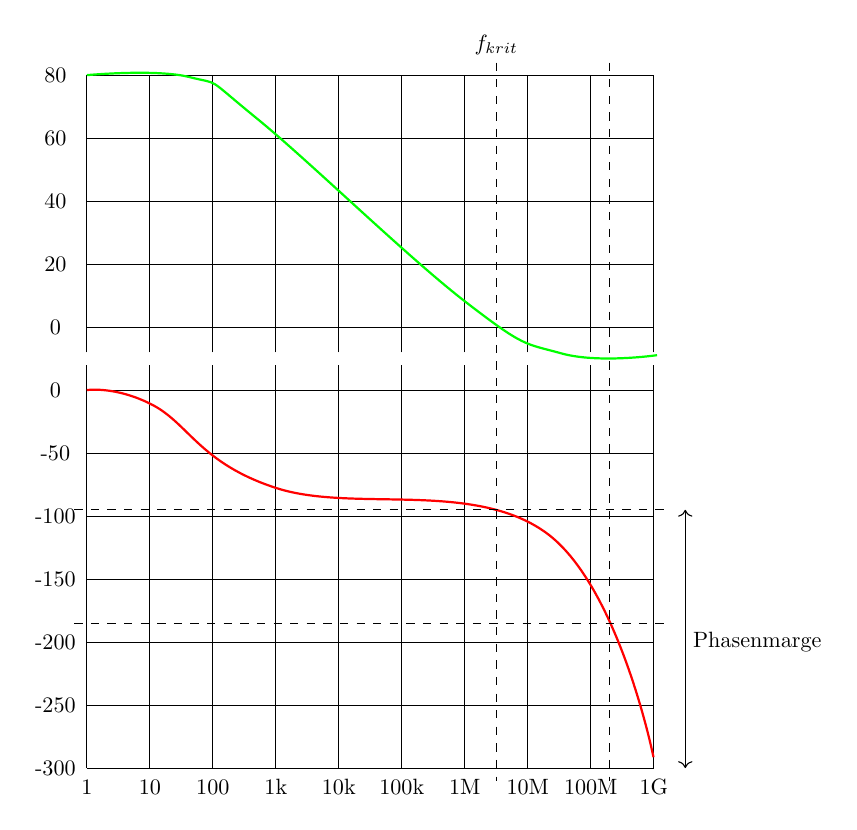
\begin{tikzpicture}[scale=0.8,transform shape]
	%axis
	%x
	\foreach \x in {0,...,9} {
		\draw (\x,0) -- (\x,6.4);
		\draw (\x,6.6) -- (\x,11);
	}
	%y
	\foreach \y in {0,...,11} {
		\draw (0,\y) -- (9,\y);
	}
	\draw node at (0,-0.3) {1};
	\draw node at (1,-0.3) {10};
	\draw node at (2,-0.3) {100};
	\draw node at (3,-0.3) {1k};
	\draw node at (4,-0.3) {10k};
	\draw node at (5,-0.3) {100k};
	\draw node at (6,-0.3) {1M};
	\draw node at (7,-0.3) {10M};
	\draw node at (8,-0.3) {100M};
	\draw node at (9,-0.3) {1G};
	
	\draw node at (-0.5,0) {-300};
	\draw node at (-0.5,1) {-250};
	\draw node at (-0.5,2) {-200};
	\draw node at (-0.5,3) {-150};
	\draw node at (-0.5,4) {-100};
	\draw node at (-0.5,5) {-50};
	\draw node at (-0.5,6) {0};
	\draw node at (-0.5,7) {0};
	\draw node at (-0.5,8) {20};
	\draw node at (-0.5,9) {40};
	\draw node at (-0.5,10) {60};
	\draw node at (-0.5,11) {80};

\draw [thick, red] plot[smooth, tension=.7] coordinates {(0,6) (1.0379,5.7673) (3.0063,4.4457) (7.2804,3.7427) (8.9957,0.1716)    };
\draw [thick, green] plot[smooth, tension=.7] coordinates {(0,11) (1.6284,10.9694) (2.697,10.314) (6.0151,7.3983) (7.5335,6.5828) (9.052,6.5547)};
\draw [dashed] (6.5,11.2) -- (6.5,-0.2);
\draw [dashed] (8.3,11.2) -- (8.3,-0.2);
\draw [dashed] (-0.2,2.3) -- (9.2,2.3);
\draw [dashed] (-0.2,4.1) -- (9.2,4.1);
\draw [<->] (9.5,4.1) -- (9.5,0);
\draw node at (9.5,2) [anchor=west] {Phasenmarge};
\draw node at (6.5,11.2) [anchor=south] {$f_{krit}$};
\end{tikzpicture}
}
		\caption{Bodeplot}
	\end{subfigure}\qquad
	\begin{subfigure}[b]{8cm}
		\centering
		{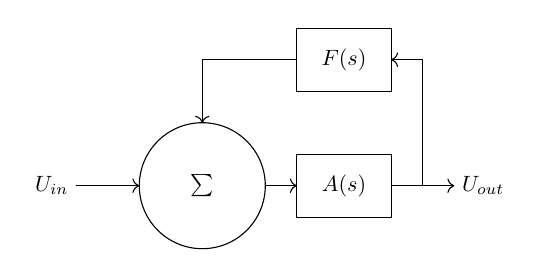
\begin{tikzpicture}[scale=0.8,transform shape]
	\draw [->] (0,0) node [anchor=east] {$U_{in}$} -- (1,0);
	\draw (2,0) circle (1);
	\draw node at (2,0) {$\sum$};
	\draw [->] (3,0) -- (3.5,0);
	\draw (3.5,0.5) rectangle (5,-0.5);
	\draw node at (4.25,0) {$A(s)$};
	\draw [->] (5,0) -- (6,0) node [anchor=west] {$U_{out}$};
	\draw [->] (5.5,0) -- (5.5,2) -- (5,2);
	\draw (5,2.5) rectangle (3.5,1.5);
	\draw node at (4.25,2) {$F(s)$};
	\draw [->] (3.5,2) -- (2,2) -- (2,1);
	

\end{tikzpicture}}
		\caption{Rückgekoppelter Verstärker}
	\end{subfigure}
	\caption{Stabilität}
	\label{fig:stabilitaet}
\end{figure}

\begin{tabular}{|l|l|}
\hline
	Phasenmarge bei $f_{krit}(a_L=1)$ &
	Verhalten des Verstärkers \\
	& (System mit zwei weit auseinanderliegenden Polen) \\\hline
	$\varphi_M \leq 0^\circ$ & 
	Gegenkoppelter Verstärker schwingt selbständig \\\hline
	$\varphi_M > 0^\circ$ &
	Gedämpftes Überschwingen der Sprungantwort \\\hline
	$\varphi_M = 65^\circ$ &
	Peaking verschwindet. Einziger Überschwinger mit 4.7\% Sprunghöhe \\\hline
	$\varphi_M \geq 75^\circ$ &
	Kein Überschwingen \\\hline
\end{tabular}

\begin{tabular}{lll}
Stabilitätskriterien & $\Phi = 180^\circ$ & $ \left|A(s)\cdot F(s)\right|<1 $ \\
& $ \left|A(s)\cdot F(s)\right|= 1 $ & $ \rightarrow 180^\circ-\Phi>0;\
\varphi_M>0^\circ $ \\
Phasenmarge & $\varphi_M=180^\circ-\Phi $ & \\
Designregel & Wähle 2. Pol ($f_nd$) bei ca. $3\cdot GBP$& \\
\end{tabular}

%\section{Gebräuchliche Realisierungen von OTA's}
%\section{Designprojekt OTA}
Vorgaben:
\begin{description}[noitemsep, leftmargin=4.2cm, style=sameline]
  \item[Open-Loop-Gain:] $\geq 80 dB$
  \item[Last:] $\leq 5 pF$
  \item[GBW:] $\geq 5 MHz$
  \item[Phase Margin:] $\geq 60^\circ$
  \item[Stabilität:] Unity-Gain stable
  \item[Slew-Rate:] $\geq 20V/\mu S$
  \item[Versorgungsspannung:] $3.3V$
  \item[Output-Swing:] (VSS + 500mV) \ldots (VDD-500mV)
\end{description}

\subsection{Design Ablauf}
OTA wird typischerweise ein Sub-Block einer grösseren Schaltung sein.

\begin{enumerate}[noitemsep]
  \item Definition der Ein- und Ausgägne einer Schaltung (Spezifikation der Schaltung)
  \item Handberechnung, Erstellung des Schaltplanes
  \item Schaltkreissimulation
  \item Erfüllt der Schaltkreis die Spezifikation? Wenn nein, zurück zu 1. Sonst weiter.
  \item Layout
  \item Schaltkreissimulation mit parasitären Einflüssen
  \item Erfüllt der Schaltkreis die Spezifikationen? Nein: Zurück zu Layout, sonst weiter.
  \item Herstellung eines Prototypen
  \item Test und Evaluation
  \item Erfüllt der Schaltkreis die Spezifikation? Nein: Zurück zur Herstellung Prototyp oder zurück zu 1.
  \item Produktion
\end{enumerate}
\section{Spannungsreferenzen}
\begin{figure}[!h]
	\centering
	\begin{subfigure}[b]{10cm}
		\centering
		{\begin{circuitikz}[scale=1.5]

\draw
	(0,0) node [ground] {}
	to [V<=$\Phi_t$] (0,1)
	to (1,1)
	(1,1.5) rectangle (2,0.5)
	(1.5,1) node {K}
	(2,1) to (3,1) to (3,1.5)
	(0,2) node [ground] {}
	to [V<=$V_D$] (0,3)
	to (3,3) to (3,2.5)
	(3,2) node {$+$} circle (0.5)
	(3.5,2) to [short] (4,2)
;

\end{circuitikz}}
		\caption{Prinzip der Spannungsreferenz}
	\end{subfigure}\qquad
	\begin{subfigure}[b]{8cm}
		\centering
		{\begin{circuitikz}[scale=1.5, european]

\draw
	(0,0) node [ground] {}
	(1,0) node [ground] {}
	(2,0) node [ground] {}
	(3,0) node [ground] {}
	(4,0) node [ground] {}
	
	(0,1) node [pnp, xscale=-1] (T1) {}
	(3,1) node [pnp] (T2) {}

	(T1.B) -| (1,0)
	(T1.C) -- (0,0)
	(T1.E) -- (0,3)
	
	(T2.B) -| (2,0)
	(T2.C) -- (3,0)
	(T2.E) to [R=$R_3$] (3,3)
	
	(1.5,4) node [op amp, rotate=90, yscale=-1] (opamp) {}
	
	(0,3) -| (opamp.+)
	(3,3) -| (opamp.-)
	
	(0,3) to [R=$R_1$, *-] (0,5) to [short, -o] (4,5)
	(3,3) to [R=$R_2$, *-*] (3,5)
	
	(opamp.out) to [short, -*] (1.5,5)
	
	(4,4.5) to (4,0.5)
	(4,2.5) node [anchor=east] {$V_{ref}$}
		
	(0.5,1.5) -- (2.5,1.5)
	
	(1.5,1.5) node [anchor=south] {$\Delta V_D$}
;

\end{circuitikz}}
		\caption{Praktische Schaltung}
	\end{subfigure}
	\caption{Bandgap-Schaltungen}
	\label{fig:spannungsreferenzen}
\end{figure}

$V_{ref}=V_D+K\cdot \Phi_t$\\
$\Phi_t = \frac{kT}{e}$, ist bei Raumtemperatur $27^\circ C$ $\Phi_t=25.9mV$\\
\begin{tabular}{ll}
Boltzmann-Konstante & $k=1.38\cdot 10^{-23}\frac{J}{K}$\\
absolute Temperatur & T = Temperatur in Kelvin\\
Elementarladung & $e=1.60\cdot 10^{-19}C$\\
\end{tabular}\\
\textbf{Realisierung:}\\
Die beiden Emitterflächen werden mit $A_1$ bzw. $A_2$ bezeichnet.\\
$V_{ref}=V_{EB1}+\Phi_t\cdot\frac{R_2}{R_3}\cdot\ln\left(\frac{R_2}{R_1}\cdot\frac{A_2}{A_1}\right)$
\end{document}
